\chapter{Methodology and Experimental Design}
%
\label{chap:Methodology}
%
This chapter describes the research design in five parts: the general approach
(Section~\ref{sec:approach}), data preparation and pattern analysis
(Section~\ref{sec:data-prep}), benchmark dataset construction
(Section~\ref{sec:benchmark}), LLM setup and prompt design
(Section~\ref{sec:llm-setup}), and the experimental protocol
(Section~\ref{sec:experimental-protocol}).

%----------------------------------------------------------------------
\section{General Approach}
\label{sec:approach}
%
The thesis follows a three-phase methodology:

\begin{enumerate}
    \item \textbf{Preprocessing.}  Raw ticket files~(MSG, PDF, DOCX, XLSX)
          are converted to a unified Markdown~(\texttt{.md}) representation.
          Structured fields are extracted with regular expressions; the remaining
          narrative text is retained for LLM processing.

    \item \textbf{Benchmark construction.}  A representative sample of
          250~tickets is drawn so that it reflects the diversity of the full
          archive.  Tickets are selected to vary along three dimensions: the
          complexity of the ticket, approximated by the number of MSG email
          files it contains; the language of the content; and the year of
          origin, spanning 2016 to 2025.  Each selected ticket is then annotated
          with ground-truth tags by a human expert.

    \item \textbf{LLM evaluation.}  Fifteen model configurations are run on each
          benchmark ticket and asked to generate tags for the ticket.  The
          generated tags are scored against the human annotations using the F1
          score, and the quality and usefulness of the tags are additionally
          assessed with an LLM-as-judge rubric.
\end{enumerate}

%----------------------------------------------------------------------
\section{Data Preparation and Pattern Analysis}
\label{sec:data-prep}
%
\subsection{Source Data}
%
The corpus consists of service tickets exported from the Amazone~Werke
service system.  Each ticket is stored as a folder containing one or more
files.  The folder name encodes the ticket identifier~(e.g.~\texttt{T250001234})
and is grouped under a parent category prefix~(\texttt{T16}--\texttt{T25},
corresponding to years 2016 to 2025).

\subsubsection{Corpus Volume and Growth}
%
Figures~\ref{fig:gs-trend}--\ref{fig:lb-trend} show the file format
composition trend for each ticket category over the period 2016 to 2025.  The
corpus has grown significantly since~2020, with PDF files dominating
Gutschrift tickets (99\%+) and MSG files becoming increasingly prominent in
Belastungsanzeige and Lagerbelastung tickets from T24~onwards.

\begin{figure}[H]
    \centering
    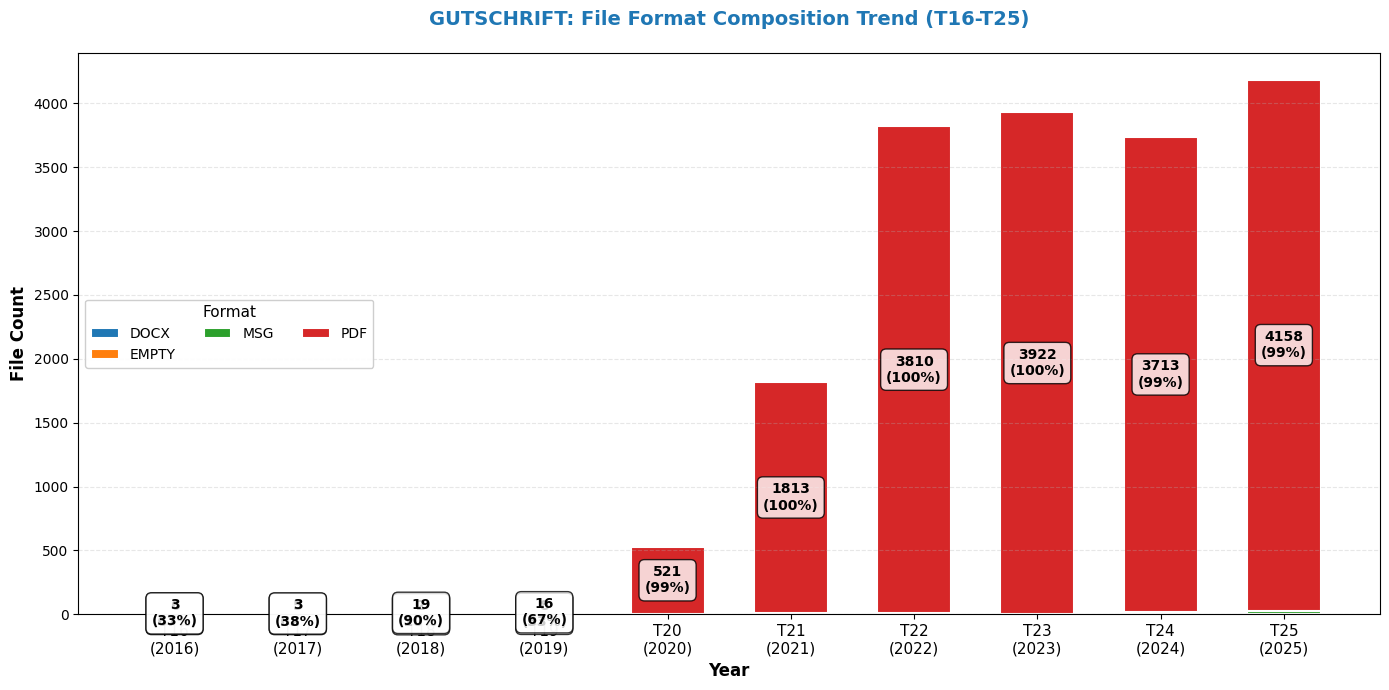
\includegraphics[width=\textwidth]{figures/gutschrift_file_format_trend.png}
    \caption[Gutschrift: file format composition trend]{Gutschrift: file format composition trend (2016 to 2025).}
    \label{fig:gs-trend}
\end{figure}

\begin{figure}[H]
    \centering
    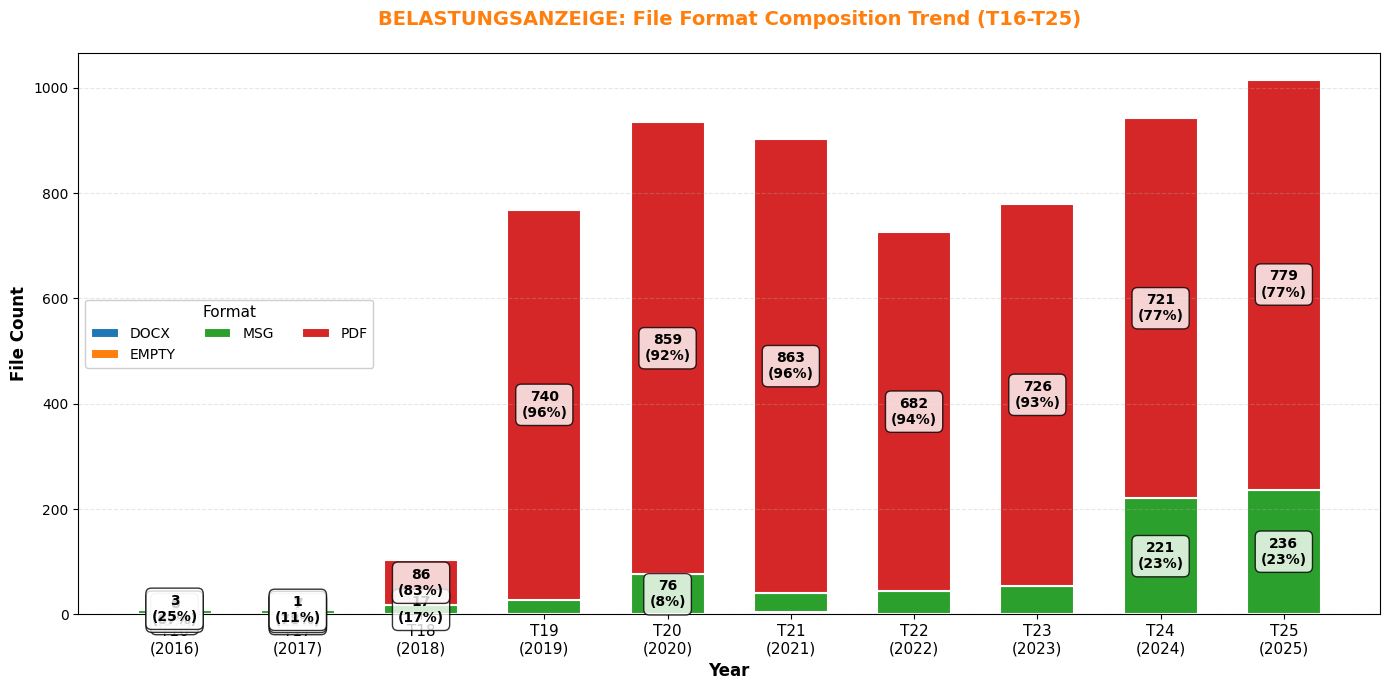
\includegraphics[width=\textwidth]{figures/belastungsanzeige_file_format_trend.png}
    \caption[Belastungsanzeige: file format composition trend]{Belastungsanzeige: file format composition trend (2016 to 2025).}
    \label{fig:bl-trend}
\end{figure}

\begin{figure}[H]
    \centering
    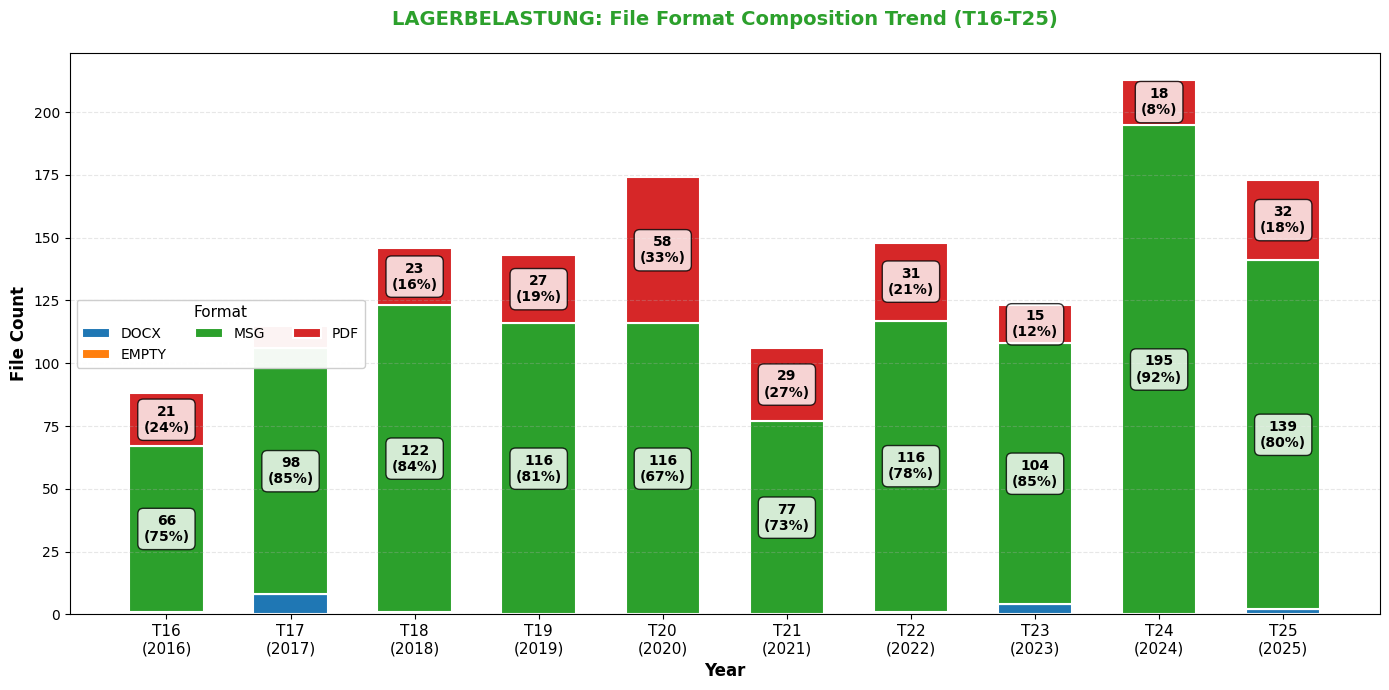
\includegraphics[width=\textwidth]{figures/lagerbelastung_file_format_trend.png}
    \caption[Lagerbelastung: file format composition trend]{Lagerbelastung: file format composition trend (2016 to 2025).}
    \label{fig:lb-trend}
\end{figure}

Figures~\ref{fig:gs-records}--\ref{fig:lb-records} show the number of
records per year for each category.  An important caveat applies to all of
these year-by-year figures: the data only becomes reliable from~2022 onwards.
Before that year, the company used a different process for recording and
archiving service tickets, so the lower record counts in the earlier years
reflect incomplete digital capture rather than a genuine absence of service
activity.  The sharp increase visible around 2021 and 2022 is therefore largely
an artefact of this process change, and any trend analysis should focus on the
period from 2022 onwards.

\begin{figure}[H]
    \centering
    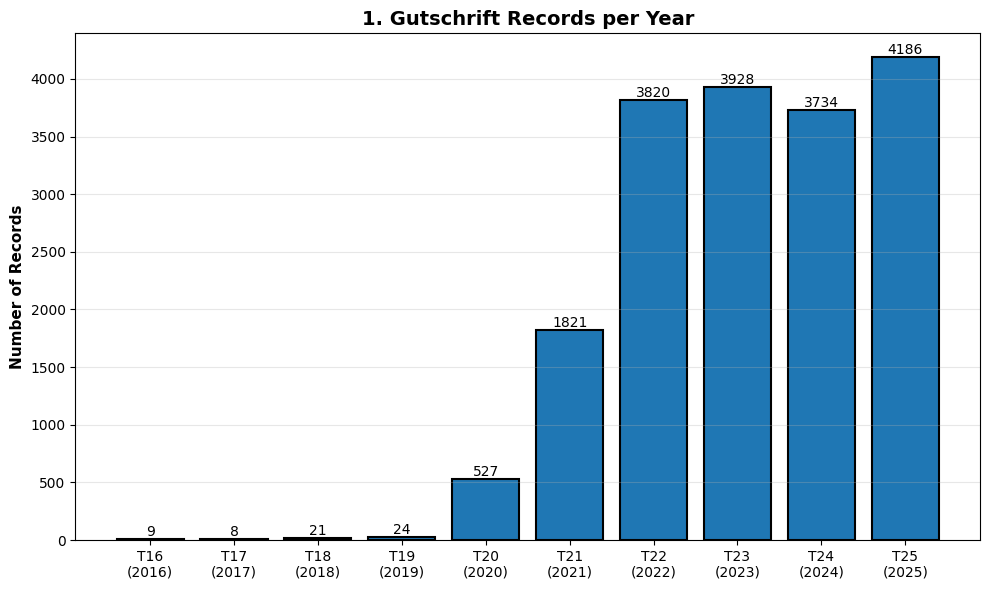
\includegraphics[width=\textwidth]{figures/gutschrift_records_per_year.png}
    \caption[Gutschrift records per year]{Gutschrift records per year (2016 to 2025). Data from 2022 onwards
             is reliable; earlier years are affected by a change in the
             company's recording process.}
    \label{fig:gs-records}
\end{figure}

\begin{figure}[H]
    \centering
    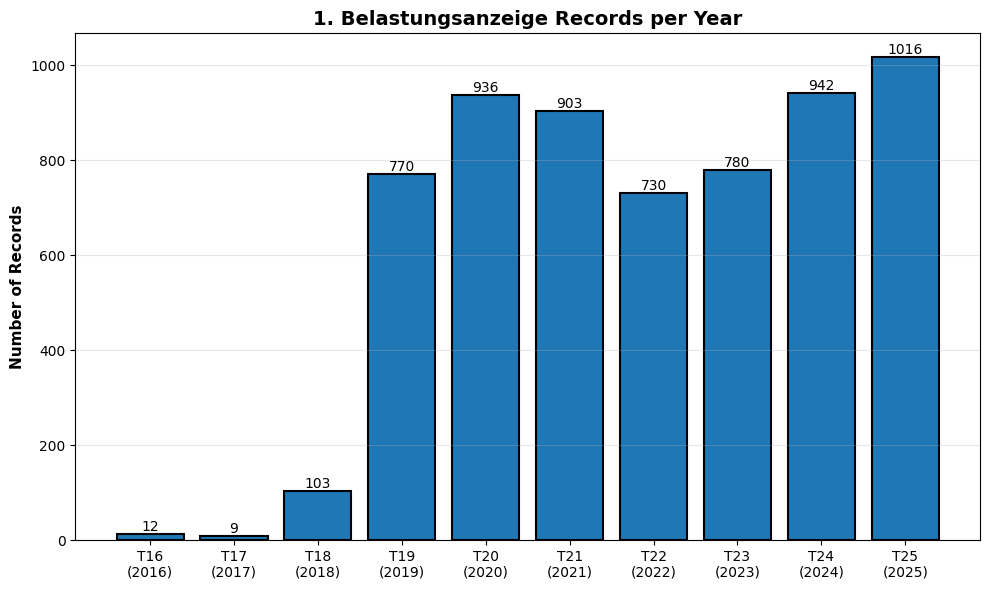
\includegraphics[width=\textwidth]{figures/belastungsanzeige_records_per_year.png}
    \caption[Belastungsanzeige records per year]{Belastungsanzeige records per year (2016 to 2025). Data from 2022
             onwards is reliable; earlier years are affected by a change in the
             company's recording process.}
    \label{fig:bl-records}
\end{figure}

\begin{figure}[H]
    \centering
    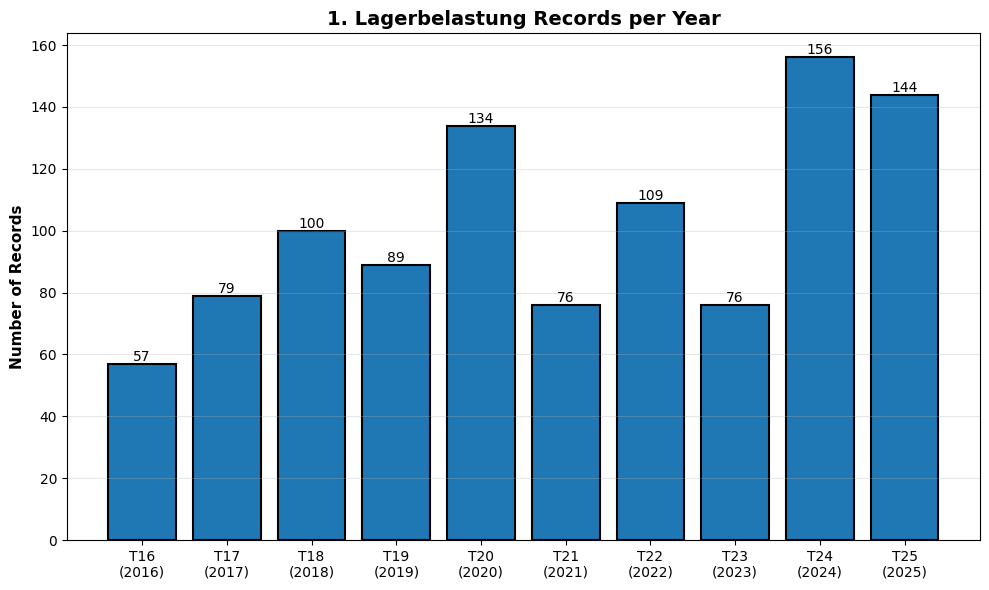
\includegraphics[width=\textwidth]{figures/lagerbelastung_records_per_year.png}
    \caption[Lagerbelastung records per year]{Lagerbelastung records per year (2016 to 2025). Data from 2022
             onwards is reliable; earlier years are affected by a change in the
             company's recording process.}
    \label{fig:lb-records}
\end{figure}

Figure~\ref{fig:gs-money} shows the total monetary value of Gutschrift
credit notes per year, peaking at over 9.1~million~EUR in 2023.
Figure~\ref{fig:bl-cost} shows the total cost per year for Belastungsanzeige
charge notifications.  The same reliability caveat applies: only the values
from~2022 onwards should be treated as representative.

\begin{figure}[H]
    \centering
    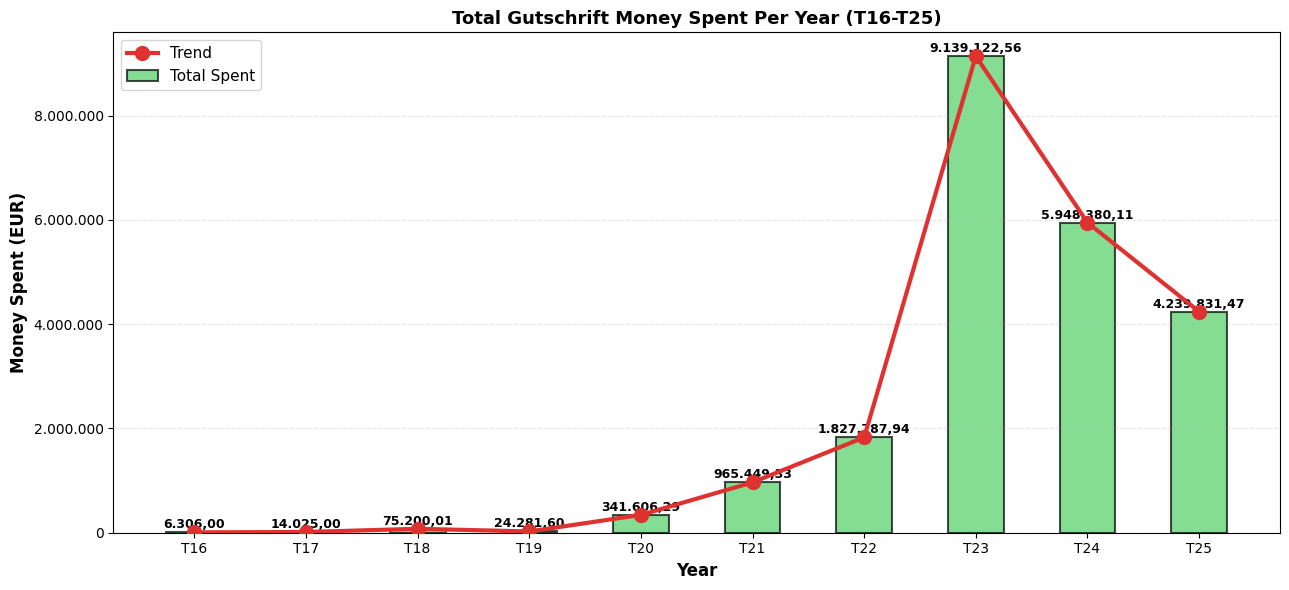
\includegraphics[width=\textwidth]{figures/gutschrift_money_spent.png}
    \caption[Total Gutschrift credit note value per year]{Total Gutschrift credit note value per year in EUR (2016 to 2025). The monetary values shown were extracted automatically with regular expressions and have not been independently verified.}
    \label{fig:gs-money}
\end{figure}

\begin{figure}[H]
    \centering
    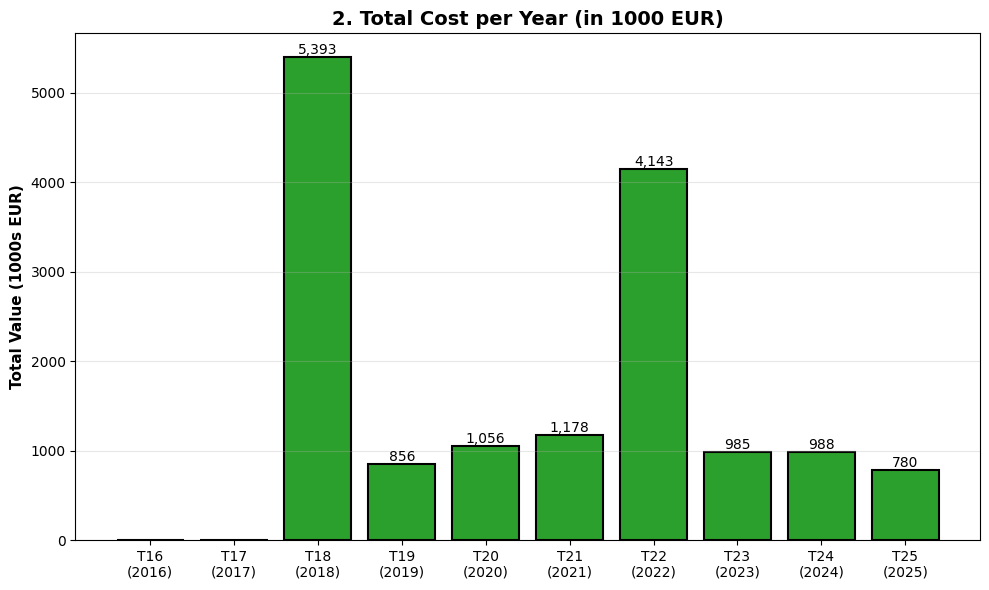
\includegraphics[width=\textwidth]{figures/belastungsanzeige_cost_per_year.png}
    \caption[Total Belastungsanzeige cost per year]{Total Belastungsanzeige cost per year in 1000~EUR (2016 to 2025). The monetary values shown were extracted automatically with regular expressions and have not been independently verified.}
    \label{fig:bl-cost}
\end{figure}

\subsection{File Conversion to Markdown}
%
All attachment types are converted to plain Markdown to create a uniform
input format for the LLM.  The conversion is performed by a custom pipeline
built for this thesis, which calls a dedicated library for each file type and
then post-processes the result.  The conversion strategy is:

\begin{itemize}
    \item MSG~(email) files: headers~(From, To, Subject, Date)
          are extracted and appended as a structured preamble, and the email body
          is normalised to plain text.  Nested reply chains are concatenated
          in chronological order (oldest first).  A custom filter in the
          pipeline removes quoted text in deep threads to reduce token
          redundancy; this filtering is part of the pipeline and is not done by
          any external conversion tool.

    \item PDF files: text is extracted using PyMuPDF4LLM, which
          preserves table structure and avoids common layout artefacts.
          Pages are separated by horizontal rules.  For scanned documents that
          contain no machine-readable text, the pipeline falls back to optical
          character recognition with Tesseract; this fallback is invoked by the
          pipeline itself, not by PyMuPDF4LLM.
\end{itemize}

\subsubsection{PDF Extraction Tool Selection}
%
The initial extraction attempts used MarkItDown~\cite{markitdown2024},
a general-purpose file-to-Markdown converter.  However, MarkItDown failed to
extract the ticket content in a correctly structured manner.  As shown in
Figure~\ref{fig:markitdown-drawback}, the converter linearises the document
into a flat sequence of fragments: column headers~(\texttt{POS},
\texttt{NO.\,D'ARTICLE}, \texttt{QUANT.}) are separated from their
corresponding values, and the tabular relationship between an article number,
its description, and its price is lost entirely.  Compared to the original PDF
layout, the extracted text is no longer
machine-interpretable as a structured invoice, which makes downstream entity
extraction unreliable.

\begin{figure}[H]
    \centering
    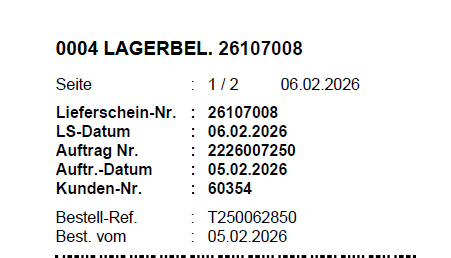
\includegraphics[width=0.82\textwidth]{figures/markitdown_drawback_output.png}\\[1ex]
    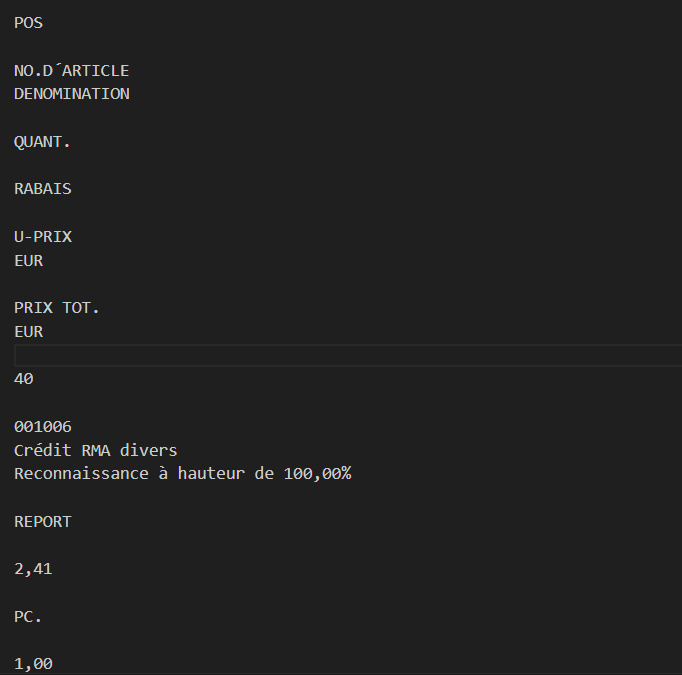
\includegraphics[width=0.82\textwidth]{figures/markitdown_drawback_original.png}
    \caption{Drawback of MarkItDown (example).  Top: the unstructured, linearised
             output, where table columns are detached from their values.
             Bottom: the original PDF layout that should have been preserved.
             These images are illustrative examples taken from one sample
             document.}
    \label{fig:markitdown-drawback}
\end{figure}

Motivated by this failure, four alternative libraries were evaluated on a test
set of 15~PDFs (5~Gutschrift, 5~Lagerbelastung, 5~Belastungsanzeige).  Before
presenting the comparison, it is worth briefly introducing these tools.  Tabula
is an open-source library specialised in detecting and extracting tables from
PDF documents.  Docling is an open-source document-conversion toolkit from IBM
that parses a PDF into a structured representation and exports it to Markdown or
JSON.  Spire.PDF is a commercial library for reading and manipulating PDF files,
including text and table extraction.  PyMuPDF4LLM is a wrapper around the PyMuPDF
engine that converts PDF pages to Markdown in a form intended for large language
model input.  A tool scores one point per PDF where \emph{all} expected fields
are correctly extracted.  Table~\ref{tab:tool-comparison} summarises the results.

\begin{table}[H]
    \centering
    \caption[PDF extraction tool comparison]{PDF extraction tool comparison (score: number of PDFs out of~15
             from which all expected fields were correctly extracted).}
    \label{tab:tool-comparison}
    \begin{tabular}{llcl}
        \hline
        \textbf{Library} & \textbf{License} & \textbf{Score} & \textbf{Cost} \\
        \hline
        PyMuPDF4LLM & AGPL       & \textbf{15/15} & Free (if not hosted) \\
        Docling      & MIT        & 11/15          & Free \\
        Spire        & Commercial & 11/15          & Paid \\
        Tabula-py    & MIT        & 6/15           & Free \\
        \hline
    \end{tabular}
\end{table}

Each tool exhibited a characteristic failure mode:

\begin{itemize}
    \item Tabula (6/15).  Tabula is specialised for table extraction
          and performed well \emph{only} on the tabular regions of a document.
          As shown in Figure~\ref{fig:tool-tabula}, it correctly reconstructs
          the key-value table~(Lieferschein-Nr., LS-Datum, Auftrag~Nr.) but
          populates many cells with \texttt{nan} and ignores all
          non-tabular text, so most documents were only partially captured.

    \item Docling (11/15).  Docling produced output that was often
          similar to the unstructured MarkItDown result.  As shown in
          Figure~\ref{fig:tool-docling}, when configured for table extraction
          it linearised the fields into separate lines and, on the 5~test PDFs
          checked specifically for table fidelity, it missed the tables in CSV
          form.

    \item Spire (11/15).  Spire matched Docling's score but, like
          MarkItDown, frequently returned a flat, unstructured stream of
          values~(Figure~\ref{fig:tool-spire}).  It is also a commercial,
          paid library.

    \item PyMuPDF4LLM (15/15).  PyMuPDF4LLM~\cite{pymupdf4llm} was the
          only tool to achieve a perfect score across all three document
          categories.  As shown in Figure~\ref{fig:tool-pymupdf4llm}, it
          preserves both the header block and the tabular structure as proper
          Markdown tables, keeping article numbers, descriptions, and prices in
          their correct relationship.
\end{itemize}

\begin{figure}[H]
    \centering
    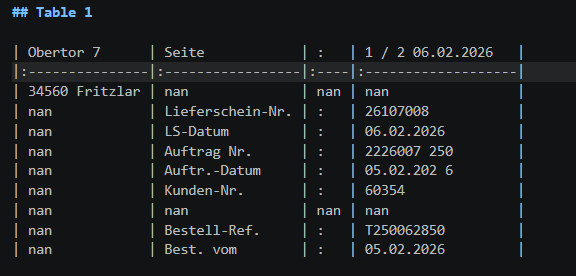
\includegraphics[width=0.92\textwidth]{figures/tool_tabula.png}
    \caption{Tabula output. Tables are reconstructed but many cells are
             \texttt{nan} and non-tabular text is dropped.}
    \label{fig:tool-tabula}
\end{figure}

\begin{figure}[H]
    \centering
    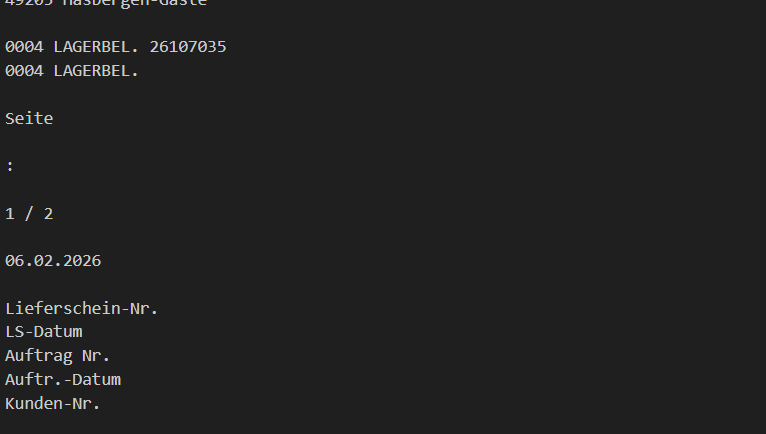
\includegraphics[width=0.92\textwidth]{figures/tool_docling.png}
    \caption{Docling output. Fields are linearised and table structure
             is lost when exporting to CSV.}
    \label{fig:tool-docling}
\end{figure}

\begin{figure}[H]
    \centering
    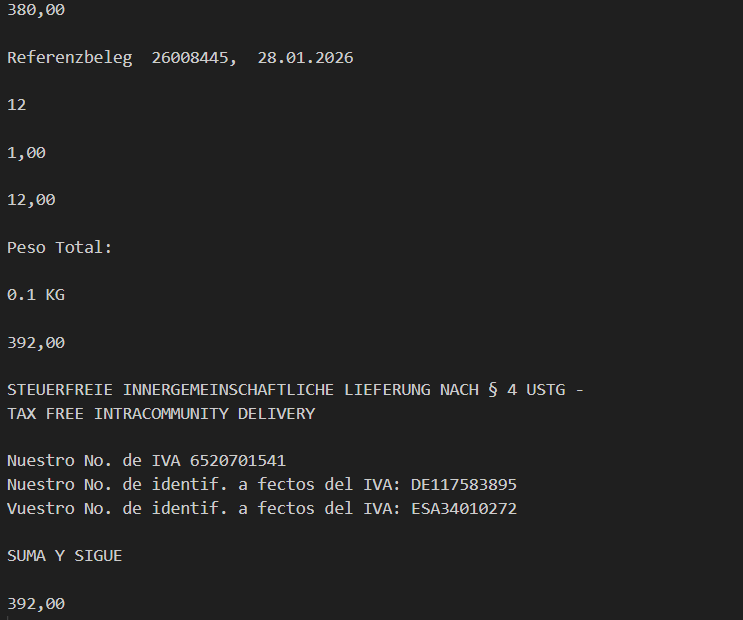
\includegraphics[width=0.85\textwidth]{figures/tool_spire.png}
    \caption{Spire output. A flat, unstructured stream of values
             similar to MarkItDown.}
    \label{fig:tool-spire}
\end{figure}

\begin{figure}[H]
    \centering
    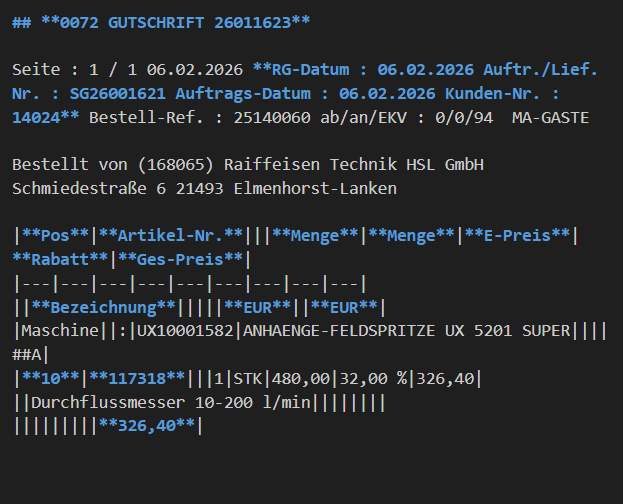
\includegraphics[width=0.92\textwidth]{figures/tool_pymupdf4llm.png}
    \caption{PyMuPDF4LLM output. Header block and tabular structure are
             preserved as proper Markdown tables.}
    \label{fig:tool-pymupdf4llm}
\end{figure}

Based on this comparison, PyMuPDF4LLM was selected as the PDF extraction tool
for the entire pipeline.  Files that cannot be converted~(corrupted,
password-protected, image-only PDFs) are skipped and logged; the remaining text
files are combined into a single \texttt{.msg.md} file per ticket.

\subsection{Token Budget Management and Cleaning}
\label{subsec:cleaning}
%
Given the 128k context window of the target models, most email threads fit
entirely.  However, to improve reasoning performance and reduce noise, a
cleaning pass is applied.  The following boilerplate patterns were identified
and removed automatically:

\begin{table}[H]
    \centering
    \caption{Most frequent boilerplate patterns removed during preprocessing.}
    \label{tab:boilerplate}
    \begin{tabular}{lr}
        \hline
        \textbf{Pattern} & \textbf{Files affected} \\
        \hline
        KG Legal Footer             & 86,408 \\
        Bank Details Block          & 84,108 \\
        AMAZONE Postal Header       & 78,073 \\
        Manufacturer Header         & 69,074 \\
        OS Trademark Notice         & 17,516 \\
        AMAZONE Standalone Address  & 13,304 \\
        urldefense URL              & 12,099 \\
        SafeLinks URL               &  8,323 \\
        IBAN Lines                  &  5,144 \\
        AMAZONE GDPR Notice DE      &  2,860 \\
        \hline
    \end{tabular}
\end{table}

\noindent
The pattern names in Table~\ref{tab:boilerplate} refer to recurring blocks of
text that were observed repeatedly across the corpus and carry no
ticket-specific information.  For example, the \emph{KG Legal Footer} is the
standard company legal footer (the firm's full legal name and registration
details) that appears at the bottom of almost every document, the \emph{Bank
Details Block} is the recurring bank-account section, and the \emph{AMAZONE
Postal Header} is the fixed sender address line.  These blocks were identified
by inspecting the most frequent repeated text segments in the benchmark data and
were removed automatically so that they do not consume context or add noise.

The combined preprocessing results are:

\begin{table}[H]
    \centering
    \caption{Preprocessing compression results.}
    \label{tab:compression}
    \begin{tabular}{lr}
        \hline
        \textbf{Metric} & \textbf{Value} \\
        \hline
        Files scanned        & 242,499 \\
        Image-only deleted   & 11,917 \\
        Files compressed     & 216,246 \\
        Files unchanged      & 14,336 \\
        Errors               & 0 \\
        \hline
        Original size        & 949.9\,MB \\
        Space saved          & 219.5\,MB \\
        Reduction            & 23.1\% \\
        \hline
    \end{tabular}
\end{table}

\subsection{Rule-based Pattern Extraction}
\label{subsec:regex}
%
An analysis of the documents revealed three recurring structured document
categories that can be identified reliably with regular expressions.  Because
the corpus is multilingual, the classifier does not rely on a single German
keyword but on a list of category keywords in several languages, combined with a
filename heuristic.  A document is assigned to a category if either its filename
matches a category-specific pattern or its first part matches a content pattern
built from the multilingual keyword list.

\begin{description}
    \item[Gutschrift~(Credit Note):] the filename pattern is
          \verb|gutschrift|credit.*note|, and the content pattern requires a
          four-digit number followed by a credit-note keyword such as
          \texttt{GUTSCHRIFT}, \texttt{CREDIT NOTE}, \texttt{NOTE DE
          CR\'EDIT}, \texttt{NOTA DI CREDITO}, or their equivalents in the
          other corpus languages.

    \item[Belastungsanzeige~(Charge Notification):] the filename pattern is
          \verb|belastung|debit.*note|, and the content pattern matches a
          debit-note keyword such as \texttt{BELASTUNGSANZEIGE}, \texttt{DEBIT
          NOTE}, \texttt{NOTE DE D\'EBIT}, or \texttt{NOTA DI ADDEBITO}.

    \item[Lagerbelastung~(Warehouse Charge):] the filename pattern is
          \verb|lagerbelastung|lager|warehouse.*debit|stock.*debit|, and the
          content pattern matches a stock-charge keyword such as
          \texttt{LAGERBELASTUNG}, \texttt{STOCK DEBIT}, or \texttt{WAREHOUSE
          DEBIT}.
\end{description}

The monetary total of a document is captured with a dedicated pattern that
looks for a total-value label such as \texttt{Gesamtwert}, \texttt{Total},
\texttt{Montant total}, or \texttt{Valor total}, followed within a short window
by a currency amount.  The amount is then parsed from the European number
format~(for example \texttt{1.234,56}) into a numeric value.

Beyond document-category detection and totals, the pipeline extracts the
identifiers that follow predictable patterns:

\begin{itemize}
    \item Machine serial numbers, matched by prefixed digit patterns such as
          \verb|UX\d{7,}| and \verb|CYA\d{7,}|.
    \item Article numbers, matched as digit sequences appearing in a part-list
          context.
    \item Change numbers~(Anderungsnummer), matched by \verb|CN[A-Z]?\d{4,}|,
          which also captures variants such as \texttt{CNY0001440}.
\end{itemize}

This rule-based layer addresses RQ\,1.1 directly: structured, pattern-conformant
information is captured without an LLM.  The LLM is reserved for extracting
the semantic tags from the narrative text.

\subsection{Item Extraction}
\label{subsec:item-extraction}
%
Applying the rule-based layer to the full corpus produces a structured record of
the items mentioned in each document.  Three kinds of identifier are of
particular interest: the article numbers (Artikel-Nr.), the customer's own part
number (Ihre Teilenummer), and the change numbers (Anderungsnummer, prefixed
with \texttt{CN}).  Because the three document categories follow different
layouts, these identifiers are stored in slightly different fields per category:
the Gutschrift and Lagerbelastung documents expose a single list of article
numbers, whereas the Belastungsanzeige documents separate the internal part
number from the customer's own part number.

Table~\ref{tab:item-extraction} summarises the volume of extracted identifiers.
The Gutschrift category dominates the article counts, with a single article
number (\texttt{0520700}) appearing more than 88{,}000 times, which reflects a
small number of very high-volume spare parts.  The change numbers are far less
frequent but are operationally important, since they link a ticket to a specific
engineering change.

\begin{table}[H]
    \centering
    \caption[Volume of extracted items per category]{Volume of extracted items per category. Article numbers, customer part numbers, and change numbers (CN) after applying the length and pattern filters.}
    \label{tab:item-extraction}
    \begin{tabular}{lrrrr}
        \hline
        \textbf{Category} & \textbf{Articles} & \textbf{Unique articles} & \textbf{CN total} & \textbf{CN unique} \\
        \hline
        Gutschrift        & 327{,}763 & 18{,}101 & 1{,}775 & 623 \\
        Belastungsanzeige &   4{,}868 &  1{,}537 & 3{,}288 & 934 \\
        Lagerbelastung    &   1{,}960 &  1{,}417 &       0 &   0 \\
        \hline
    \end{tabular}
\end{table}

Figure~\ref{fig:item-articles} shows the twenty most frequent article numbers in
each category.  The distribution is highly skewed for Gutschrift, where a few
standard parts account for the bulk of all occurrences, and much flatter for
Lagerbelastung, where no single part dominates.

\begin{figure}[H]
    \centering
    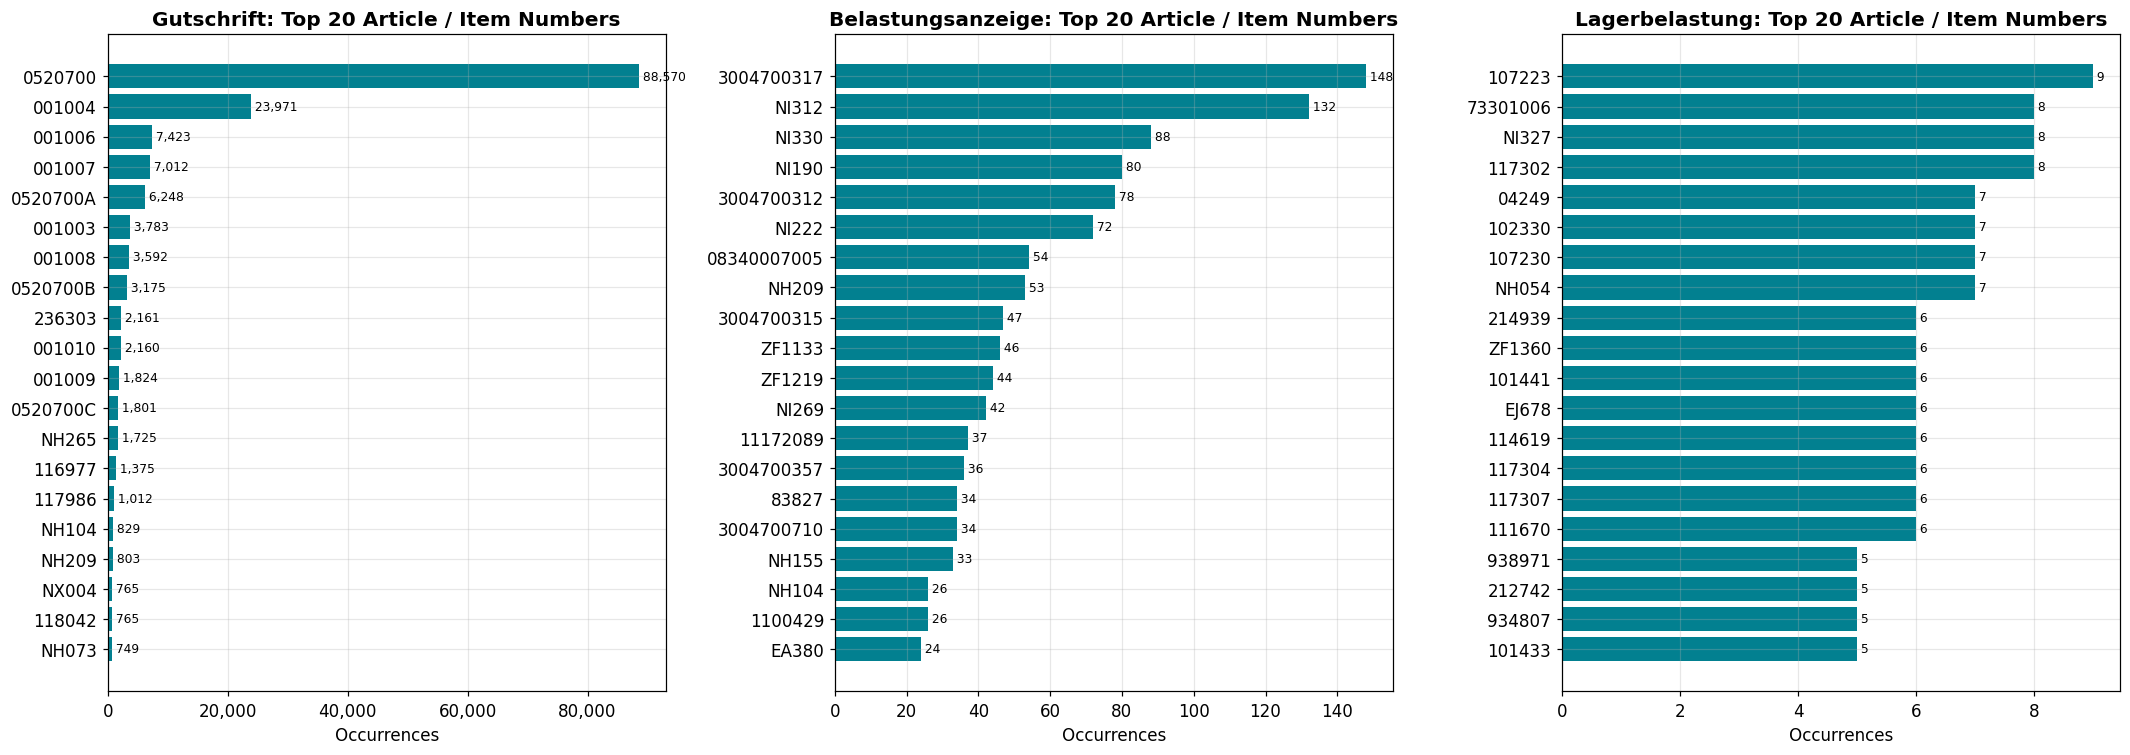
\includegraphics[width=\textwidth]{figures/fig_top_article_numbers.png}
    \caption[Top article numbers per category]{Top twenty article and item numbers per category, after filtering out change numbers and short tokens.}
    \label{fig:item-articles}
\end{figure}

For the Belastungsanzeige category, the customer's own part number is recorded in
a dedicated field.  Figure~\ref{fig:item-ihre} shows the most frequent values,
which are useful for tracing recurring customer-side components.

\begin{figure}[H]
    \centering
    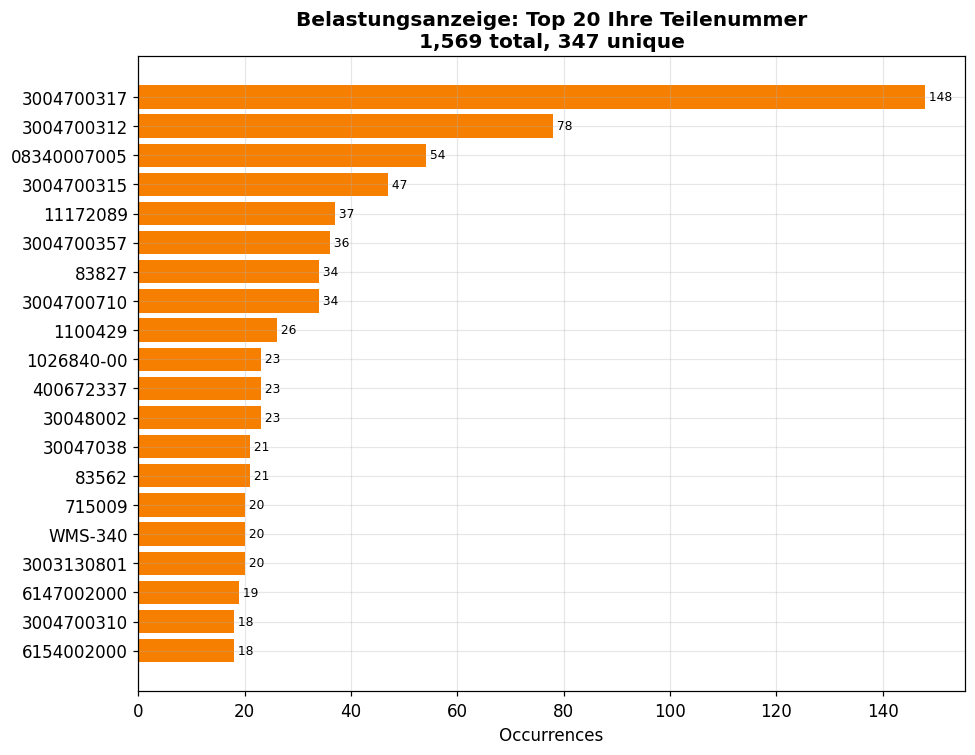
\includegraphics[width=0.78\textwidth]{figures/fig_ihre_teilenummer.png}
    \caption[Top customer part numbers]{Top twenty customer part numbers (Ihre Teilenummer) in the Belastungsanzeige category.}
    \label{fig:item-ihre}
\end{figure}

The change numbers are extracted separately and, as
Figure~\ref{fig:item-cn} shows, the sets found in the Gutschrift and
Belastungsanzeige categories are almost entirely disjoint: of the several
hundred unique change numbers in each category, only a single number appears in
both.  They are therefore presented as two separate distributions rather than a
combined one.  It is worth noting that in the Gutschrift documents the change
numbers were not isolated in a dedicated field but had to be recovered from the
surrounding text, which is a limitation of the original extraction and a
candidate for future refinement.

\begin{figure}[H]
    \centering
    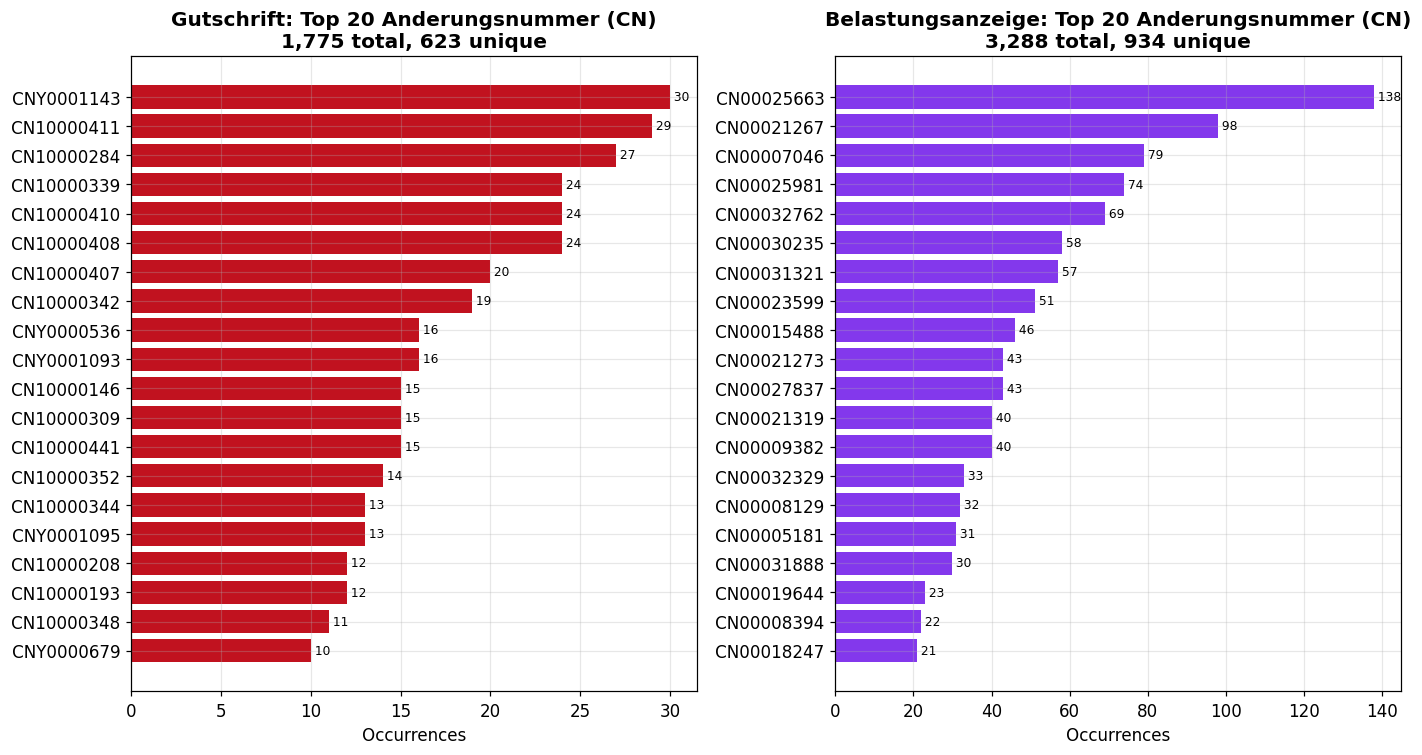
\includegraphics[width=\textwidth]{figures/fig_anderungsnummer.png}
    \caption[Change number occurrences per category]{Top twenty change numbers (Anderungsnummer, CN) for the Gutschrift and Belastungsanzeige categories, shown separately because the two sets are disjoint.}
    \label{fig:item-cn}
\end{figure}

%----------------------------------------------------------------------
\section{Benchmark Dataset and Validation}
\label{sec:benchmark}
%
\subsection{Ticket Selection}
%
A stratified sample of 250~tickets was drawn from the full corpus to represent
three distinct ticket categories:

\begin{itemize}
    \item \textbf{GS~(Gutschrift/Credit-note tickets):} Billing corrections,
          credit requests, invoice disputes.
    \item \textbf{BL~(Belastungsanzeige tickets):} Charge notifications,
          commission corrections, return-goods authorisations.
    \item \textbf{LB~(Lagerbelastung tickets):} Warehouse charges,
          stock adjustments, logistics issues.
\end{itemize}

Tickets were selected to ensure coverage of different years~(2016 to 2025),
a variety of email-thread lengths~(1 to 20+ messages), and both resolved and
unresolved cases.  The benchmark composition is 50~Gutschrift,
100~Belastungsanzeige, and 100~Lagerbelastung tickets, chosen to balance
category representation with the relative complexity of each type.

\subsubsection{Benchmark Data Characteristics}
%
The language distribution of the benchmark tickets is dominated by German
(Table~\ref{tab:language-dist}), reflecting the typical communication
patterns between Amazone's German headquarters and its international
dealer network.

\begin{table}[H]
    \centering
    \caption{Language distribution across the source files in the 250-ticket benchmark.}
    \label{tab:language-dist}
    \begin{tabular}{lrr}
        \hline
        \textbf{Language} & \textbf{Percent} & \textbf{Files} \\
        \hline
        German   & 82.8\% & 538 \\
        English  & 15.7\% & 102 \\
        Russian  &  1.1\% &   7 \\
        Spanish  &  0.3\% &   2 \\
        Estonian &  0.2\% &   1 \\
        \hline
    \end{tabular}
\end{table}

\noindent
The counts in Table~\ref{tab:language-dist} refer to individual source files,
not tickets: a single ticket bundles several files, so the file counts exceed
the 250 tickets.  German and English together account for the overwhelming
majority, with a small remainder in Russian, Spanish, and Estonian.

Figure~\ref{fig:benchmark-filetypes} shows the distribution of source file
types in the benchmark.  MSG email files dominate overwhelmingly (622~out of
650~files, 95.7\%), confirming that the primary communication channel is
email.

\begin{figure}[H]
    \centering
    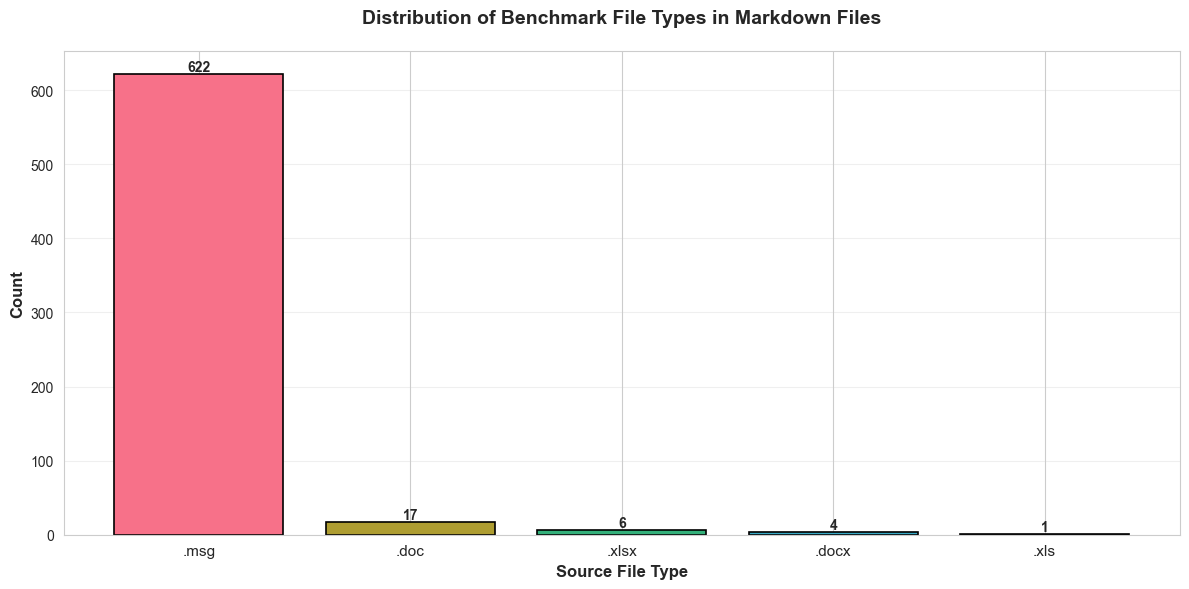
\includegraphics[width=\textwidth]{figures/benchmark_file_type_distribution.png}
    \caption{Distribution of source file types in the benchmark Markdown files.}
    \label{fig:benchmark-filetypes}
\end{figure}

Figure~\ref{fig:ticket-classification} shows that 237~tickets~(97.1\%)
contain at least one \texttt{.msg.md} file, while only 7~tickets~(2.9\%)
consist entirely of non-email files.

\begin{figure}[H]
    \centering
    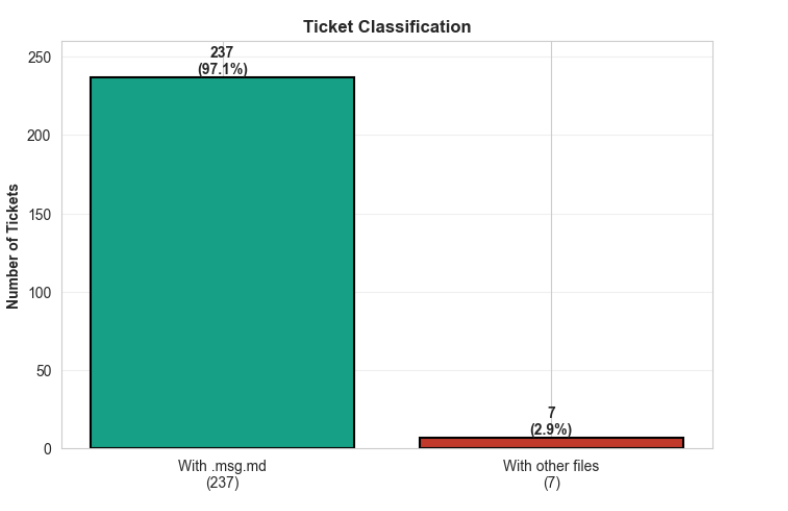
\includegraphics[width=0.95\textwidth]{figures/ticket_classification.png}
    \caption{Ticket classification: tickets with .msg.md files vs other files only.}
    \label{fig:ticket-classification}
\end{figure}

Figure~\ref{fig:files-per-ticket} shows the distribution of files per
ticket.  The majority of tickets (60.7\%) contain only a single file, while
4.9\% contain eleven or more files, representing complex multi-message
threads with attachments.

\begin{figure}[H]
    \centering
    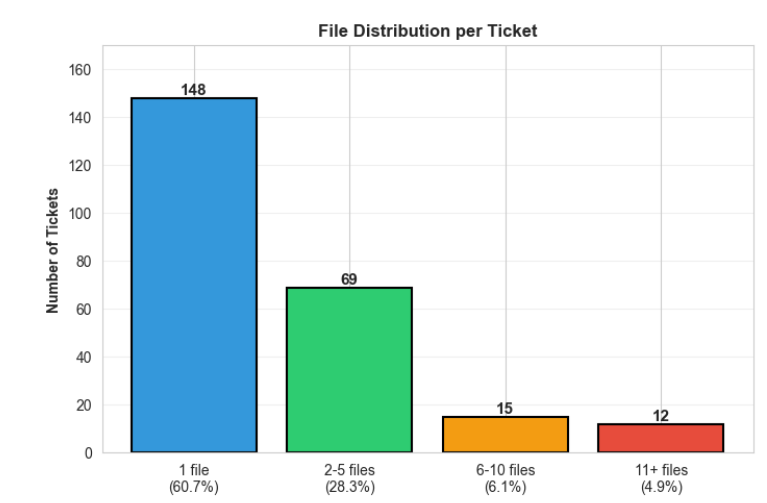
\includegraphics[width=\textwidth]{figures/file_distribution_per_ticket.png}
    \caption{Distribution of files per ticket in the benchmark dataset.}
    \label{fig:files-per-ticket}
\end{figure}

\subsection{Human Annotation}
%
Each ticket was annotated by a single domain expert with knowledge of
Amazone's service operations.  The annotation task consisted of assigning
1 to 4 tags to each ticket from a curated set of 28 human-defined tags, for
example \texttt{kulanz}, \texttt{wrong\_booking}, and \texttt{discussion}.

These 28~tags form the human-annotated ground truth used in the F1 evaluation.
They were developed manually by working through the benchmark tickets and
grouping the most common and clearly recurring service themes into reusable
labels.  The tags are intentionally coarse-grained and service-action-oriented
to maximise reusability across similar tickets.

This human-defined set was later extended into a larger taxonomy of
126~tags for the blind tag evaluation.  The extension was driven by the
language models themselves: prompting the models to generate tags freely across
the corpus produced a pool of roughly 1{,}789~candidate tags, which was then
reduced to 126~clear, non-overlapping labels through a dedicated
quality-control pass.  The full development process is described in
Section~\ref{sec:disc-tags}, and the complete 126-tag list is provided in
Appendix~\ref{chap:TagTaxonomy}.

\subsection{Annotation Quality}
%
Inter-annotator agreement was not formally measured for the full benchmark
because only one annotator was available.  However, a reliability check was
performed on 25~tickets~(10\,\% of the benchmark), where the annotator
re-labelled the same tickets two weeks after the initial annotation.
The self-agreement F1 was \(0.88\), indicating good consistency.

%----------------------------------------------------------------------
\section{LLM Setup and Prompt Design}
\label{sec:llm-setup}
%
\subsection{Model Serving Infrastructure}
%
All open-source models are served via \textbf{Ollama}~(v0.3), a lightweight
local inference server, on a dedicated GPU server~(\texttt{ve-ds-nns-01}).
The server is equipped with sufficient VRAM to run 8B to 20B parameter models
at 4-bit quantisation.  The OpenWebUI front-end is used for interactive
testing and context-window verification.

The proprietary models~(GPT-4o, GPT-3.5-Turbo, GPT-4o-mini) are accessed via
the OpenAI API.

\subsection{Models Evaluated}
%
Table~\ref{tab:models} lists all fifteen model configurations evaluated in
this thesis, spanning both open-source models served via Ollama and
proprietary models accessed via the OpenAI API.

\begin{table}[H]
    \centering
    \caption{Models evaluated in the benchmark study.}
    \label{tab:models}
    \begin{tabular}{llll}
        \hline
        \textbf{Short Name} & \textbf{Model} & \textbf{Source} & \textbf{Origin} \\
        \hline
        gptoss         & gpt-oss:20b          & Ollama  & OpenAI (USA) \\
        gemma4         & gemma4:7b             & Ollama  & Google (USA) \\
        gemma7b        & gemma:7b              & Ollama  & Google (USA) \\
        llama3.1       & llama3.1:8b           & Ollama  & Meta (USA) \\
        llama3.2       & llama3.2:latest       & Ollama  & Meta (USA) \\
        dolphin        & dolphin-mixtral       & Ollama  & Mistral AI (France) \\
        qwen3\_14b     & qwen3:14b             & Ollama  & Alibaba (China) \\
        qwen2.5        & qwen2.5:7b            & Ollama  & Alibaba (China) \\
        deepseek7b     & deepseek-r1:7b        & Ollama  & DeepSeek (China) \\
        deepseek14     & deepseek-r1:14b       & Ollama  & DeepSeek (China) \\
        gpt-5.5        & gpt-5.5               & API     & OpenAI (USA) \\
        gpt-5\_4-mini  & gpt-5.4-mini          & API     & OpenAI (USA) \\
        gpt-4o         & gpt-4o                & API     & OpenAI (USA) \\
        gpt-4o-mini    & gpt-4o-mini           & API     & OpenAI (USA) \\
        gpt-3.5-turbo  & gpt-3.5-turbo         & API     & OpenAI (USA) \\
        \hline
    \end{tabular}
\end{table}

Throughout this thesis, models are referred to by their Ollama identifier in
typewriter font, which combines the model family, its version, and its
parameter size, for example \texttt{gemma4:7b} or \texttt{deepseek-r1:14b}.
Where the parameter size is given separately, it appears in parentheses, as in
\texttt{gemma3 (12b)}.  It is important to note that the family version and the
parameter size are independent: \texttt{gemma4} and \texttt{gemma3 (12b)} are
two distinct model releases, not the same model written two ways.  This naming
convention is used consistently so that every result can be traced back to the
exact model that produced it.

\subsection{Prompt Design}
\label{sec:prompt-design}
%
Each ticket is processed with \textbf{two sequential API calls}:

\begin{enumerate}
    \item \textbf{Extraction call.}  The model receives the full ticket text
          and is instructed to return a JSON object with three fields:
          \texttt{Problem}~(one to two sentences), \texttt{Solution}~(one to two sentences),
          and \texttt{items}~(a JSON array of typed entity references).
          The prompt embeds explicit reasoning steps~(identify the problem,
          search for a solution, extract entities) to guide chain-of-thought
          processing.

    \item \textbf{Tagging call.}  The model receives the same ticket text and
          is instructed to return a JSON object with a \texttt{tags} array
          and a \texttt{reasoning} dictionary.  Tags must be drawn exclusively
          from the approved tag list; the model is penalised in the evaluation
          for invented tags.
\end{enumerate}

All prompts are written in English regardless of the ticket language.  The
instruction to output in English is repeated explicitly to counteract
the tendency of some models to mirror the input language.

Inference parameters are fixed across all models: temperature~$= 0.7$,
\texttt{num\_ctx}~$= 131{,}072$~tokens~(128k), \texttt{num\_predict}~$= 4{,}096$
tokens.  These values ensure that even the longest email threads are fully
ingested, while the output budget is generous enough to accommodate detailed
reasoning without being wastefully large.

%----------------------------------------------------------------------
\section{Experimental Protocol}
\label{sec:experimental-protocol}
%
\subsection{Pipeline Implementation}
%
The core pipeline is implemented as a single Python~3 script~(\texttt{extraction.py}).
For each row in the 250-ticket benchmark CSV, the script:

\begin{enumerate}
    \item Locates the ticket folder by matching the \texttt{parent\_name} and
          \texttt{ticket\_number} columns to the folder hierarchy on disk.
    \item Concatenates all \texttt{.msg.md} files for that ticket into one
          context string, prefixing each file's content with a
          \verb|[FILE: <name>]| header to preserve authorship context.
    \item Sends the extraction call and then the tagging call to the Ollama
          API, parses both JSON responses, and writes the results back to the
          output CSV.
    \item Saves a checkpoint every~10~rows~(\texttt{SAVE\_EVERY~=~10}) to
          prevent data loss on interruption.
\end{enumerate}

A one-second sleep is inserted between rows to reduce load on the GPU
server~\texttt{ve-ds-nns-01:11434}.
